\section{Results}

\subsection{Sensitivity analysis}

\begin{figure}
  \centering
  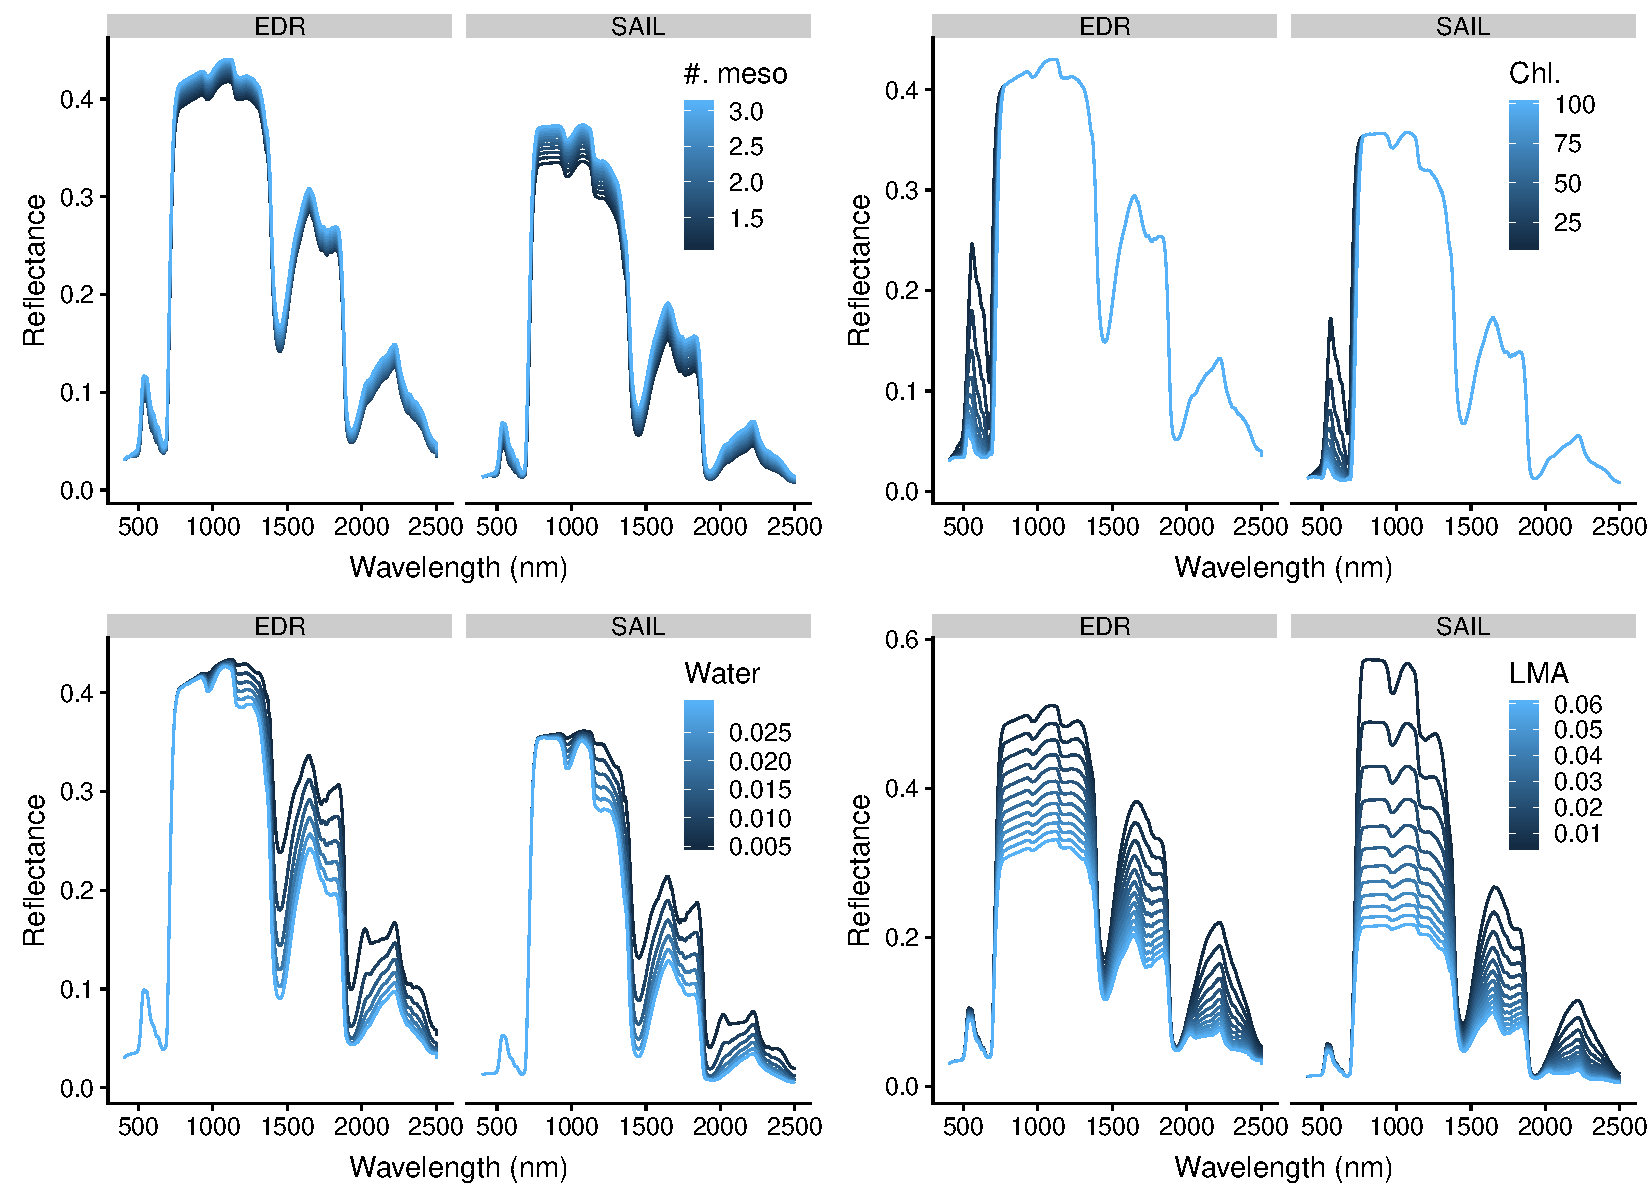
\includegraphics[width=\textwidth]{4_edr/figures/explore_spectra/edr_sensitivity_leaf_single.pdf}
  \caption{\
    Sensitivity of EDR and 4SAIL predicted canopy reflectance to leaf optical traits.
    For all figures, leaf area index is fixed at 4.88.
    EDR simulations are for a single-cohort canopy (Early Hardwood) with
    clumping factor 0.09 and orientation factor 0.06.
    4SAIL predictions are for directional-hemispherical reflectance.
  }\label{fig:sensitivity_leaf_single}
\end{figure}

The general character of the sensitivities of EDR and 4SAIL to leaf optical properties is similar,
but the magnitudes of these sensitivites are different (Figure~\ref{fig:sensitivity_leaf_single}).
EDR consistently shows significantly higher reflectance across most of the spectrum than 4SAIL\@.
Sensitivity to leaf mesophyll structure is lower in EDR than 4SAIL, while sensitivity for chlorophyll and water contents is comparable.
Sensitivity to leaf dry mass per area is comparable for both models in the shortwave infrared, but significantly higher for 4SAIL in the near infrared.

\begin{figure}
  \centering
  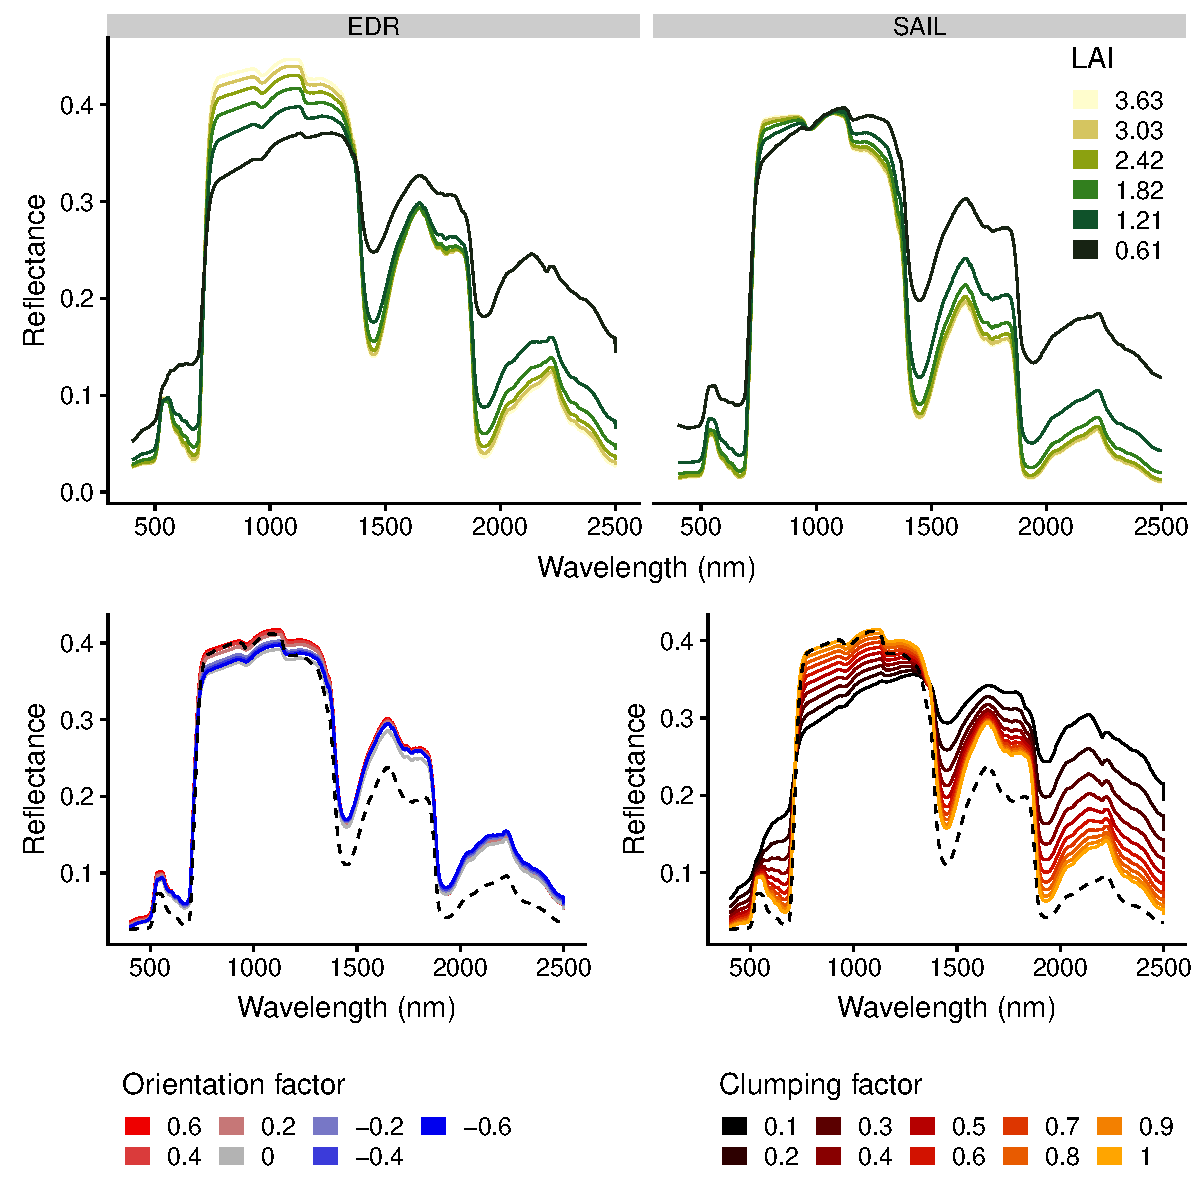
\includegraphics[width=\textwidth]{4_edr/figures/explore_spectra/sensitivity_single_pft.pdf}
  \caption{\
    Sensitivity of EDR and 4SAIL predicted canopy reflectance to leaf area index (\textit{top}) and leaf orientation factor (\textit{middle}).
    (\textit{Bottom}) Sensitivity of EDR predicted canopy reflectance and clumping factor,
    with dashed line indicating 4SAIL predictions for the same leaf area index, PROSPECT parameters, and approximately equivalent soil background.
    Configuration is the same as in Figure~\ref{fig:sensitivity_leaf_single}.
  }\label{fig:sensitivity_structure_single}
\end{figure}

EDR and 4SAIL show different responses to leaf area index (Figure~\ref{fig:sensitivity_structure_single}).
Although both models predict declines in reflectance with increasing leaf area in the visible and shortwave infrared range,
4SAIL also predicts a decline in the near infrared while EDR predicts an increase.
The sensitivities of both models to leaf area index are also different.
4SAIL predicts more reflectance sensitivity at low leaf area indices and saturation of reflectance around 4, while EDR shows a more gradual decline in sensitivity, particularly in the near-infrared range. 
Similarly to leaf area, EDR and 4SAIL agree on the directionality leaf orientation effects on reflectance (declining reflectance with increasingly vertical leaves), but differ in their sensitivities, with EDR having a much lower sensitivity to changing leaf angles.
Finally, sensitivity of EDR to canopy clumping is nearly identical to that of leaf area index, which makes sense given the interaction between these terms in defining canopy transmissivity (Equations~\ref{eq:tau_r} and~\ref{eq:tai}).

\begin{figure}
  \centering
  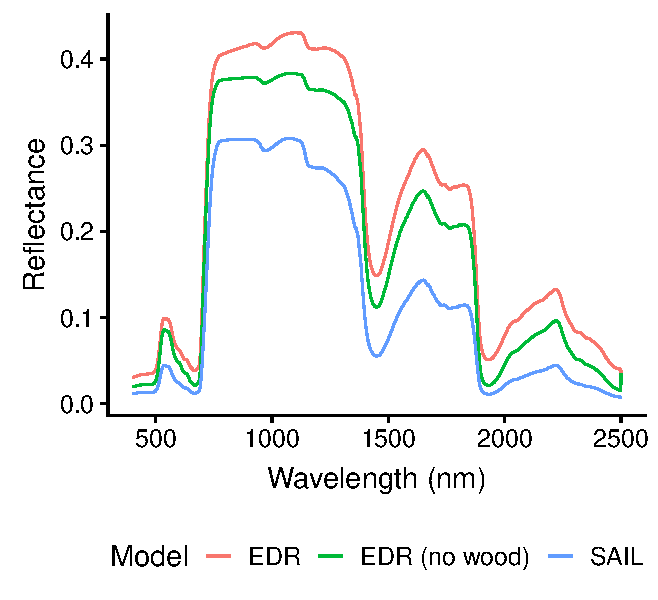
\includegraphics{4_edr/figures/explore_spectra/edr_wood_compare.pdf}
  \caption{\
    Comparison of predicted canopy reflectance by 4SAIL (directional-hemispherical) and EDR with and without wood reflectance included.
  }\label{fig:wood_compare}
\end{figure}

Compared to 4SAIL, EDR consistently overpredicts canopy reflectance across the entire spectrum (Figures~\ref{fig:sensitivity_leaf_single},~\ref{fig:sensitivity_structure_single}, and~\ref{fig:wood_compare}).
A significant part of this bias can be explained by the inclusion of wood reflectance in EDR, but a persistent positive bias remains across most of the spectrum even after setting wood reflectance to zero (Figure~\ref{fig:wood_compare}).

\begin{figure}
  \centering
  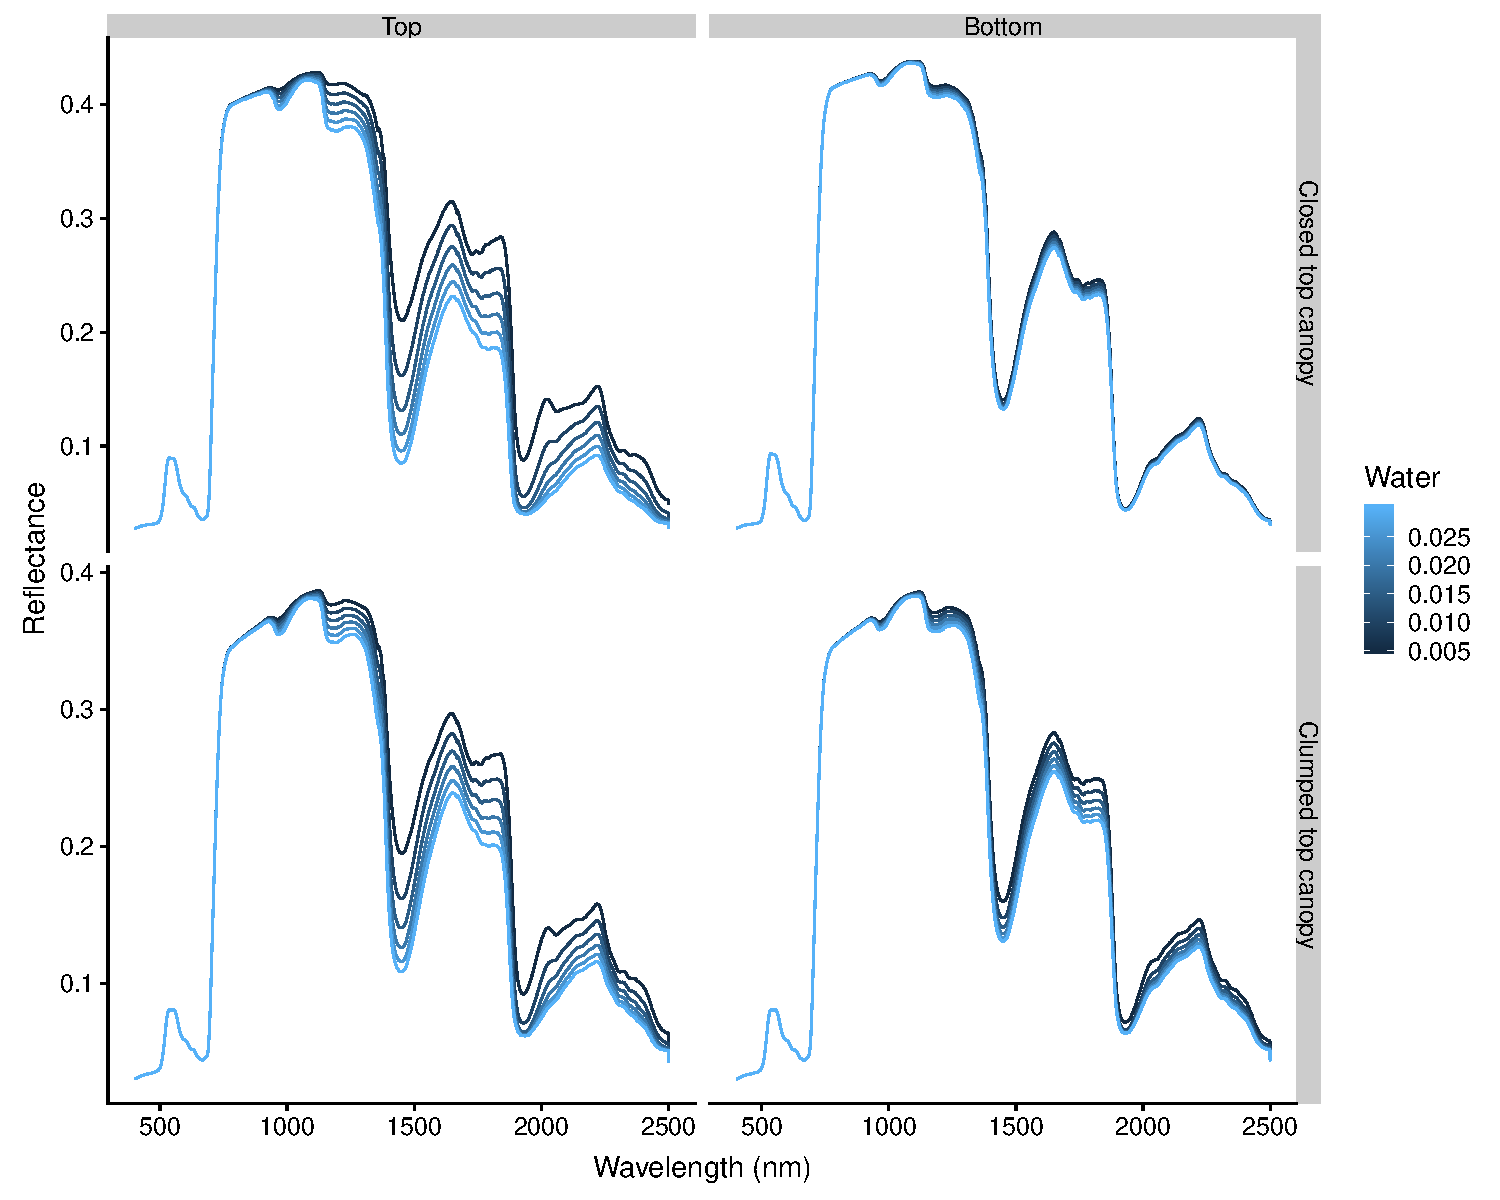
\includegraphics[width=\textwidth]{4_edr/figures/explore_spectra/edr_sensitivity_double.pdf}
  \caption{\
    Sensitivity of EDR canopy reflectance to leaf water content of top (\textit{left}) and bottom (\textit{right}) cohorts within a multi-cohort canopy,
    when the top canopy is closed (\textit{top}) and highly clumped (\textit{bottom}).
    Top and bottom cohorts are, respectively, Early and North Mid Hardwood with DBH 40 and 30, LAI 2.4 and 1.3, and equal stem density.
    Clumping factors for closed and clumped canopies are 0.9 and 0.3, respectively.
  }\label{fig:sensitivity_water_multi}
\end{figure}

EDR canopy reflectance is highly sensitive to the properties of the tallest cohort, and shows virtually no sensitivity to the optical properties of lower cohorts (Figure\ref{fig:sensitivity_water_multi}).
Clumping (or reduced LAI) allow more light to penetrate the canopy and therefore increases the sensitivity of canopy reflectance to the properties of lower layers, but this sensitivity is effect is still significantly muted compared to the top canopy.


\subsection{Model calibration}

\begin{figure}
  \centering
  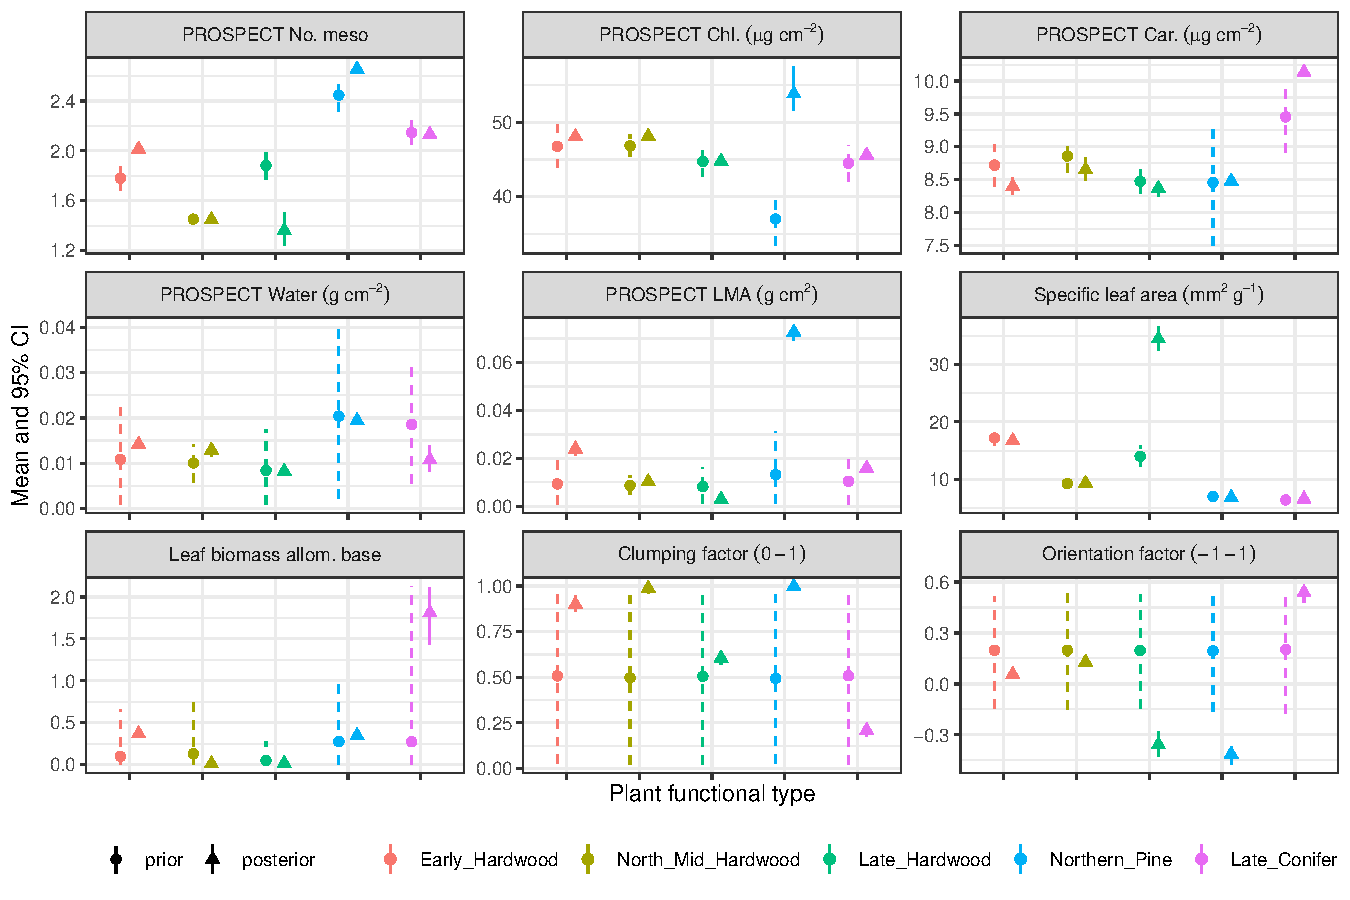
\includegraphics[width=\textwidth]{4_edr/figures/explore_spectra/pda_summary.pdf}
  \caption{\
    Summary statistics for model calibration parameter prior and posterior distributions.
  }\label{fig:pda_posteriors}
\end{figure}

Model calibration substantially improved the precision of almost all parameter estimates, even when prior distributions were strongly informative (Figure~\ref{fig:pda_posteriors}).
In most cases, the posterior distribution fell within the prior, but there were a few notable exceptions.
Specifically, northern pines had significantly higher calibration estimates of chlorophyll content and leaf mass per area and significantly lower estimates of the orientation factor (though the prior on the latter was not based on data).
Late hardwoods also had orientation factor estimates much lower than the prior, and also had significantly lower estimates of leaf mesophyll structure.

\begin{figure}
  \centering
  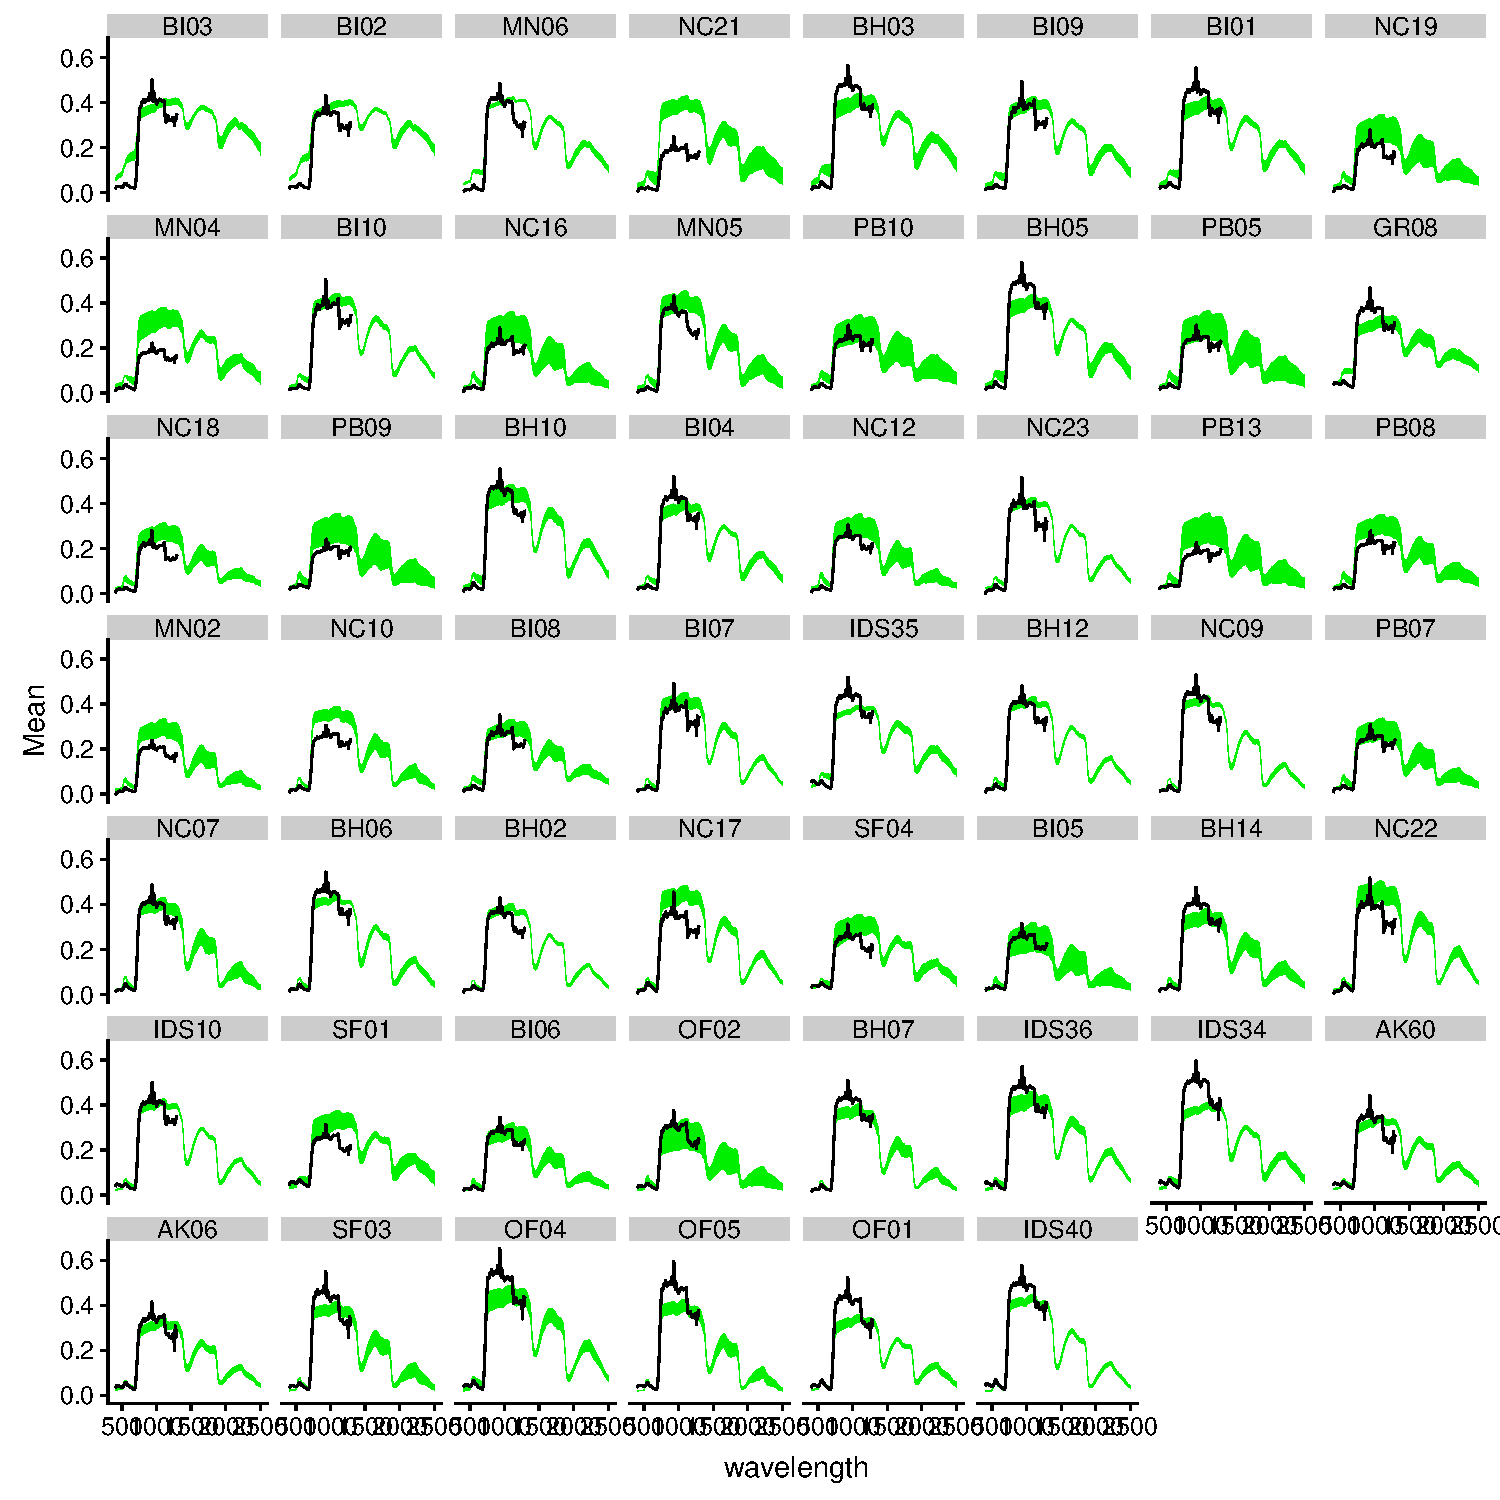
\includegraphics[width=\textwidth]{4_edr/figures/explore_spectra/errors_byvis_all.pdf}
  \caption{%
    Comparison between AVIRIS observations and posterior credible intervals on EDR predicted spectra for each site used in the calibration.
    Sites are sorted in order of decreasing mean bias in the visible ($<$750 nm) spectral region.
  }\label{fig:spec_error_all}
  % TODO: Put the CI on top, and make it transparent
  % TODO: Rotate x axis labels
\end{figure}

\begin{figure}
  \centering
  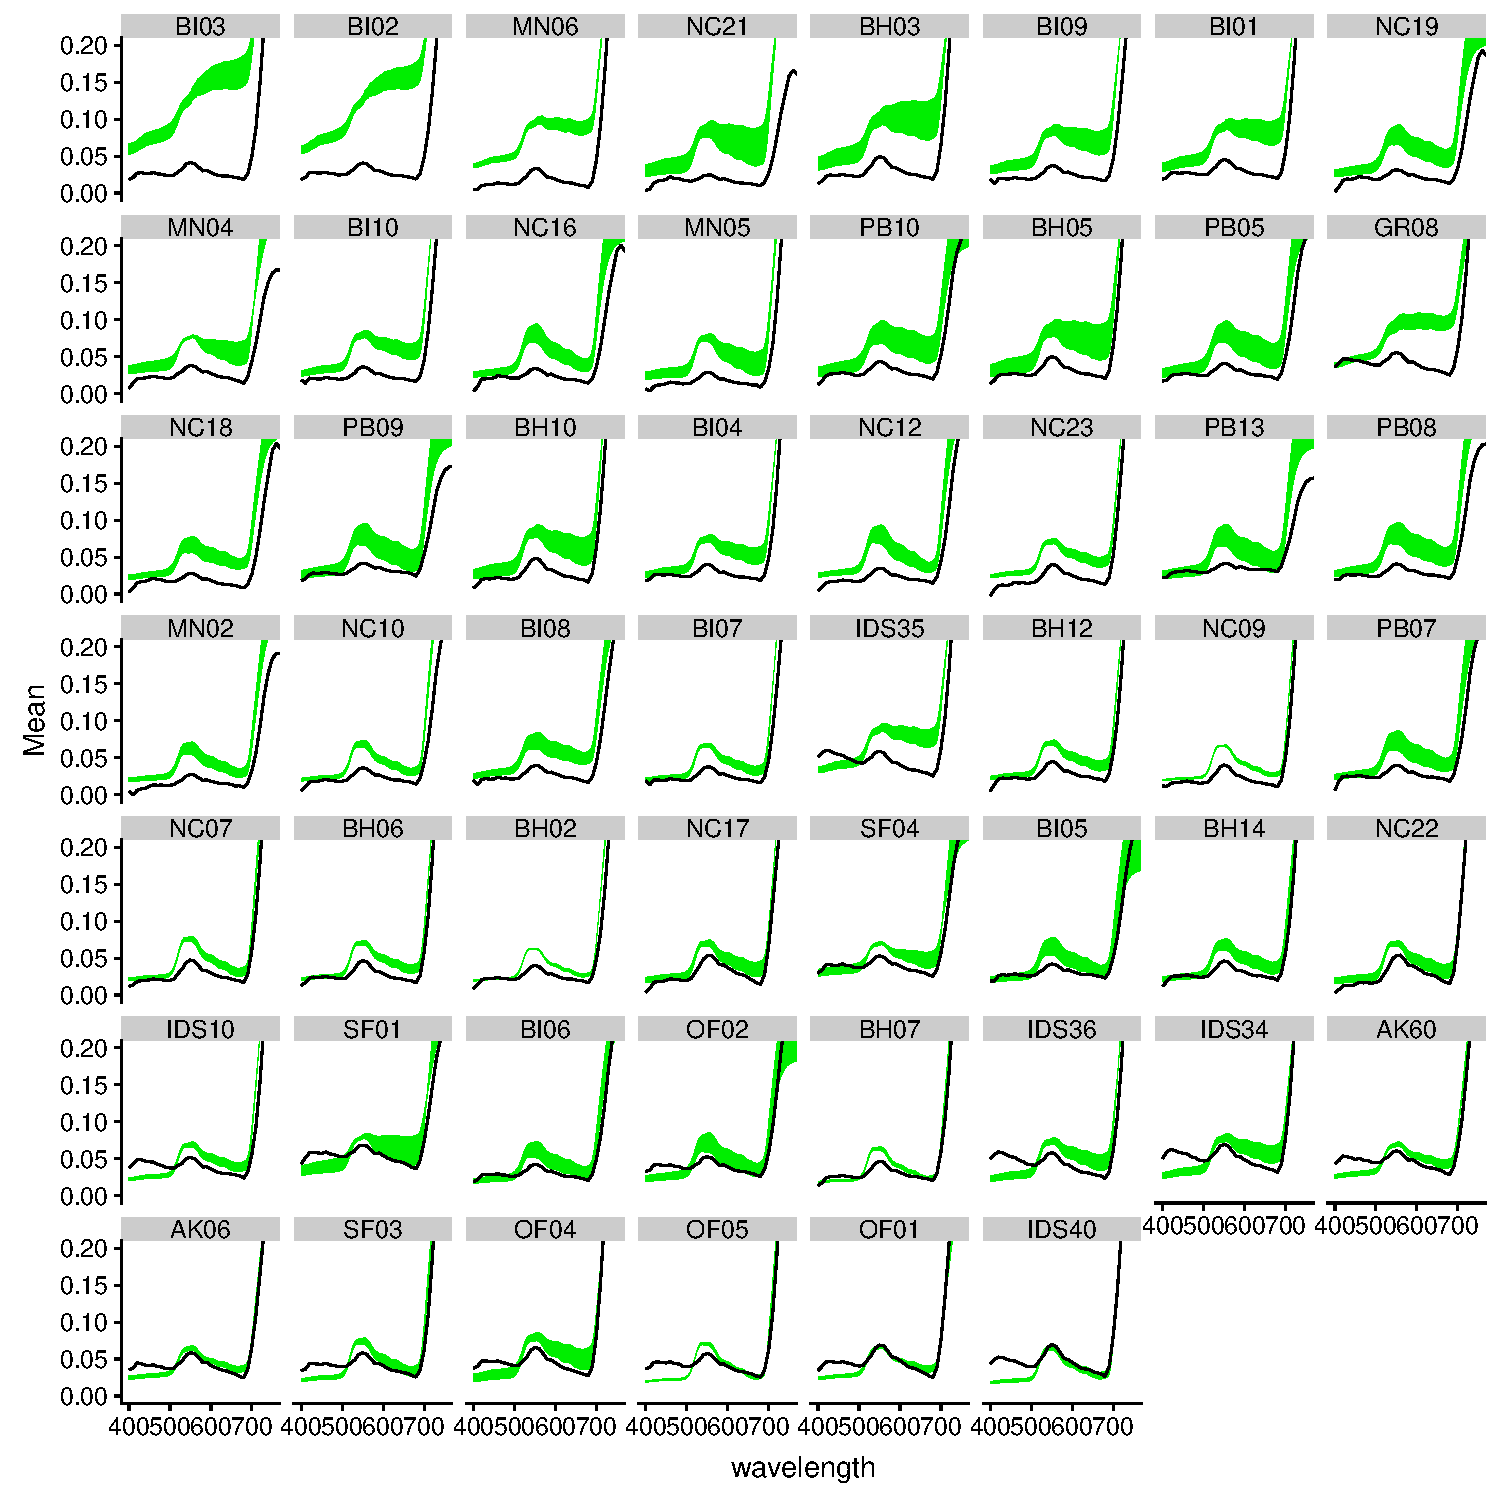
\includegraphics[width=\textwidth]{4_edr/figures/explore_spectra/errors_byvis_vis.pdf}
  \caption{%
    Same as Figure~\ref{fig:spec_error_all}, but zoomed into the visible ($<$750 nm) spectral region.
  }\label{fig:spec_error_vis}
  % TODO: Same as above
\end{figure}

\begin{figure}
  \centering
  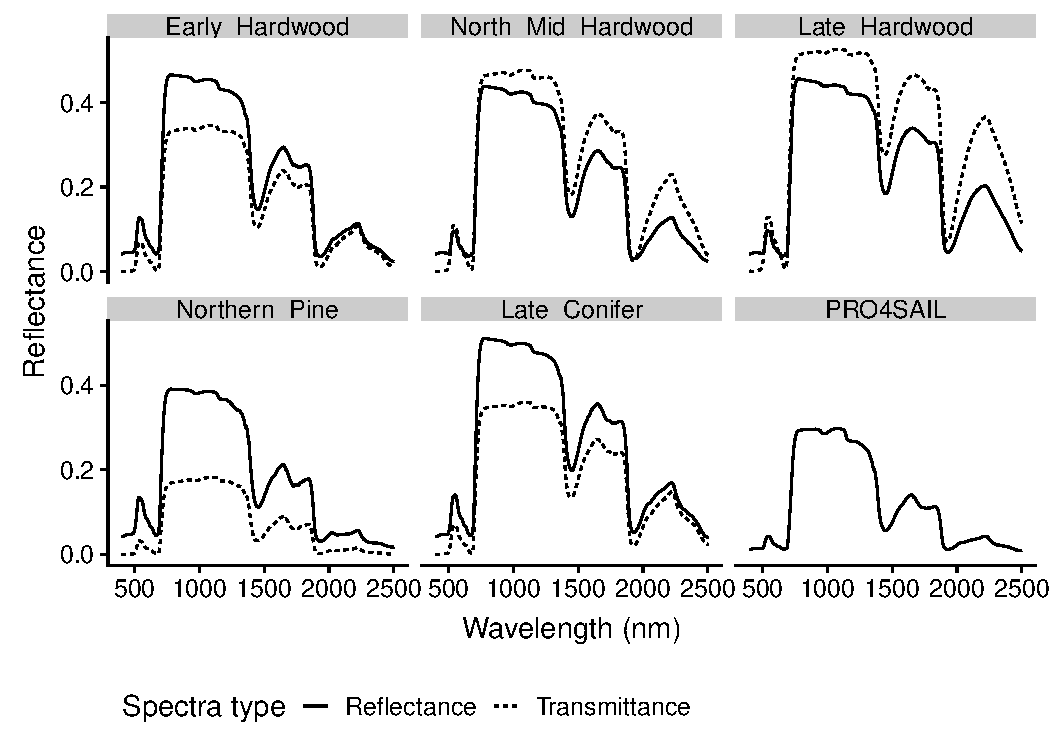
\includegraphics[width=\textwidth]{4_edr/figures/explore_spectra/pft_prospect_sim.pdf}
  \caption{%
    First five panels are PROSPECT simulations of leaf reflectance and transmittance for the plant functional types used in this analysis, based on parameters at their posterior means.
    The final panel is a simulation using the PRO4SAIL~\cite{verhoef_1984_sail} canopy radiative transfer model, parameterized with default structural parameters and leaf parameters averaged across the posterior means of the five plant functional types.
    % TODO: Add SAIL simulation
  }\label{fig:prospect_posterior}
\end{figure}

The ability of EDR to reproduce observed spectra at every site was strongly site-dependent (Figure~\ref{fig:spec_error_all}).
At a majority of the sites, EDR systematically over-predicted reflectance in the visible range (Figure~\ref{fig:spec_error_vis}), while errors in the near-infrared region were more variable.
Given that leaf transmittance is consistently lower than leaf reflectance in the visible range (Figure~\ref{fig:prospect_posterior}), this suggests that the balance of leaf reflectance and transmittance effects on canopy albedo in EDR are unbalanced in favor of the former.

%\begin{figure} \centering
  %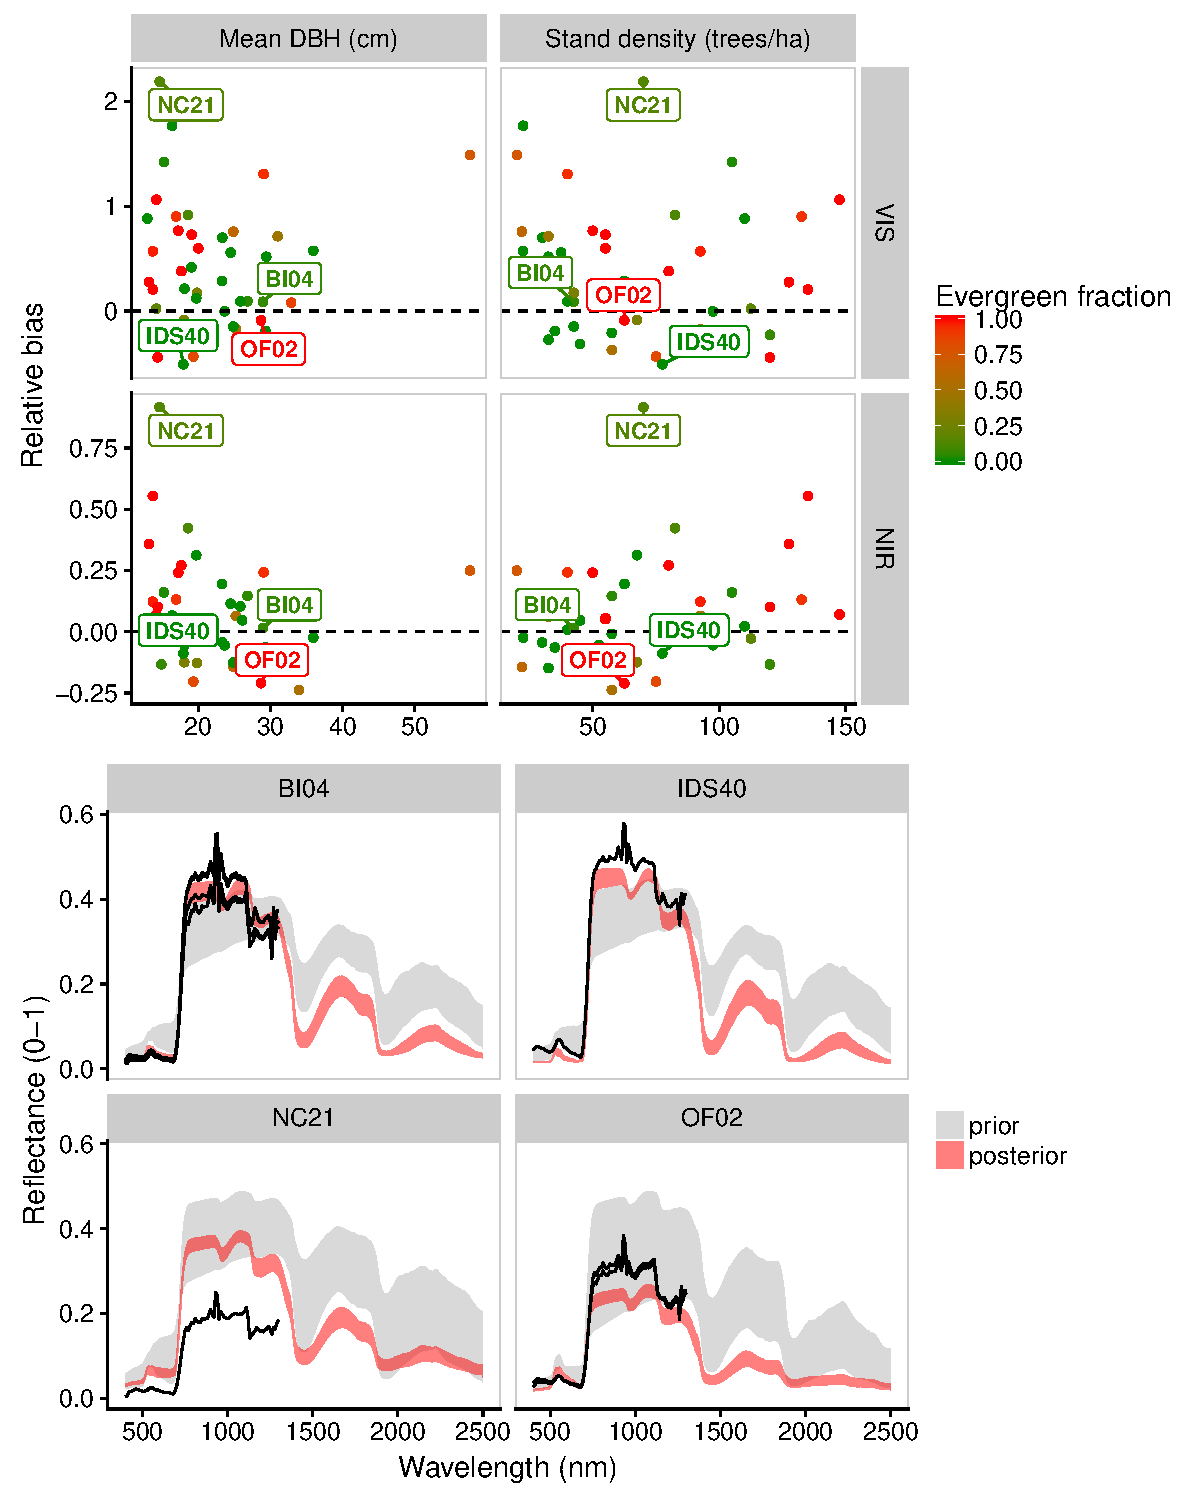
\includegraphics[width=\textwidth]{4_edr/figures/spec_validation.pdf}
  %\caption{\
    %(\textit{Top}) Relative bias of the posterior mean spectra at each site, aggregated across the visible (VIS, 400--750 nm) and near-infrared (NIR, 750--1300 nm) spectral range
    %as a function of site mean diameter at breast height and stand density.
    %(\textit{Bottom}) Prior and posterior predictive intervals and AVIRIS observations for four sites representative of different kinds of error.
  %}\label{fig:bias}
%\end{figure}

%In general, after calibration across a large number of structurally and functionally diverse sites, EDR was able to reproduce observed AVIRIS canopy reflectance reasonably well.  However, performance was strongly site specific.
%At many sites, but most prominently those composed of small trees (DBH < 20, e.g.\ site NC21), EDR frequently overestimated canopy reflectance.
%That being said, least-squares linear regressions of relative spectral bias as a function of site mean DBH or stand density were not statistically significant ($p > 0.1$).
%EDR was generally more likely to overestimate canopy reflectance for conifer trees than broadleaved trees.

\begin{figure}
  \centering
  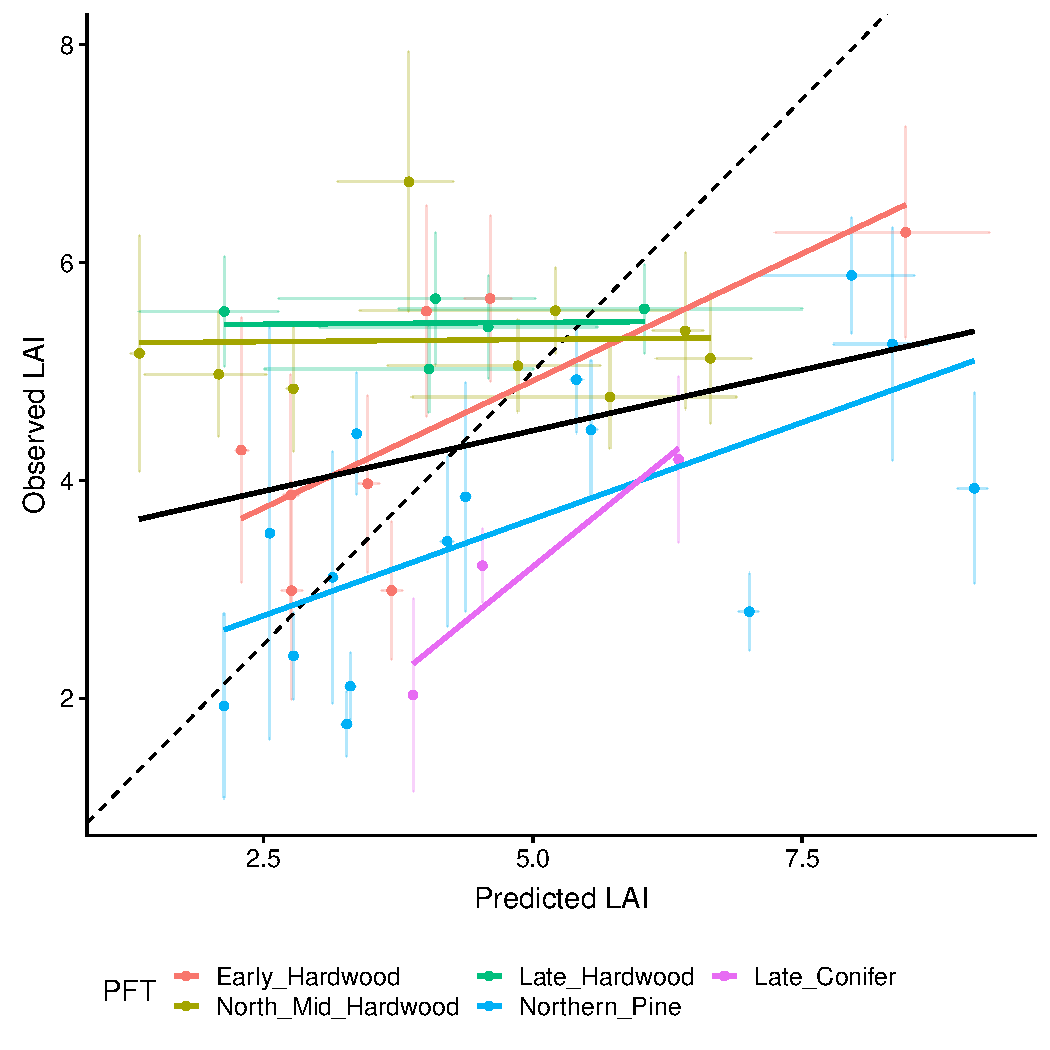
\includegraphics[width=\textwidth]{4_edr/figures/explore_spectra/lai_scatter.pdf}
  \caption{\
    Predictions of leaf area index by EDR, compared to observed values.
    Colors indicate the plant functional type of the tallest cohort at each site.
    % TODO: Add by-PFT regression line
  }\label{fig:lai_validation}
\end{figure}

\begin{figure}
  \centering
  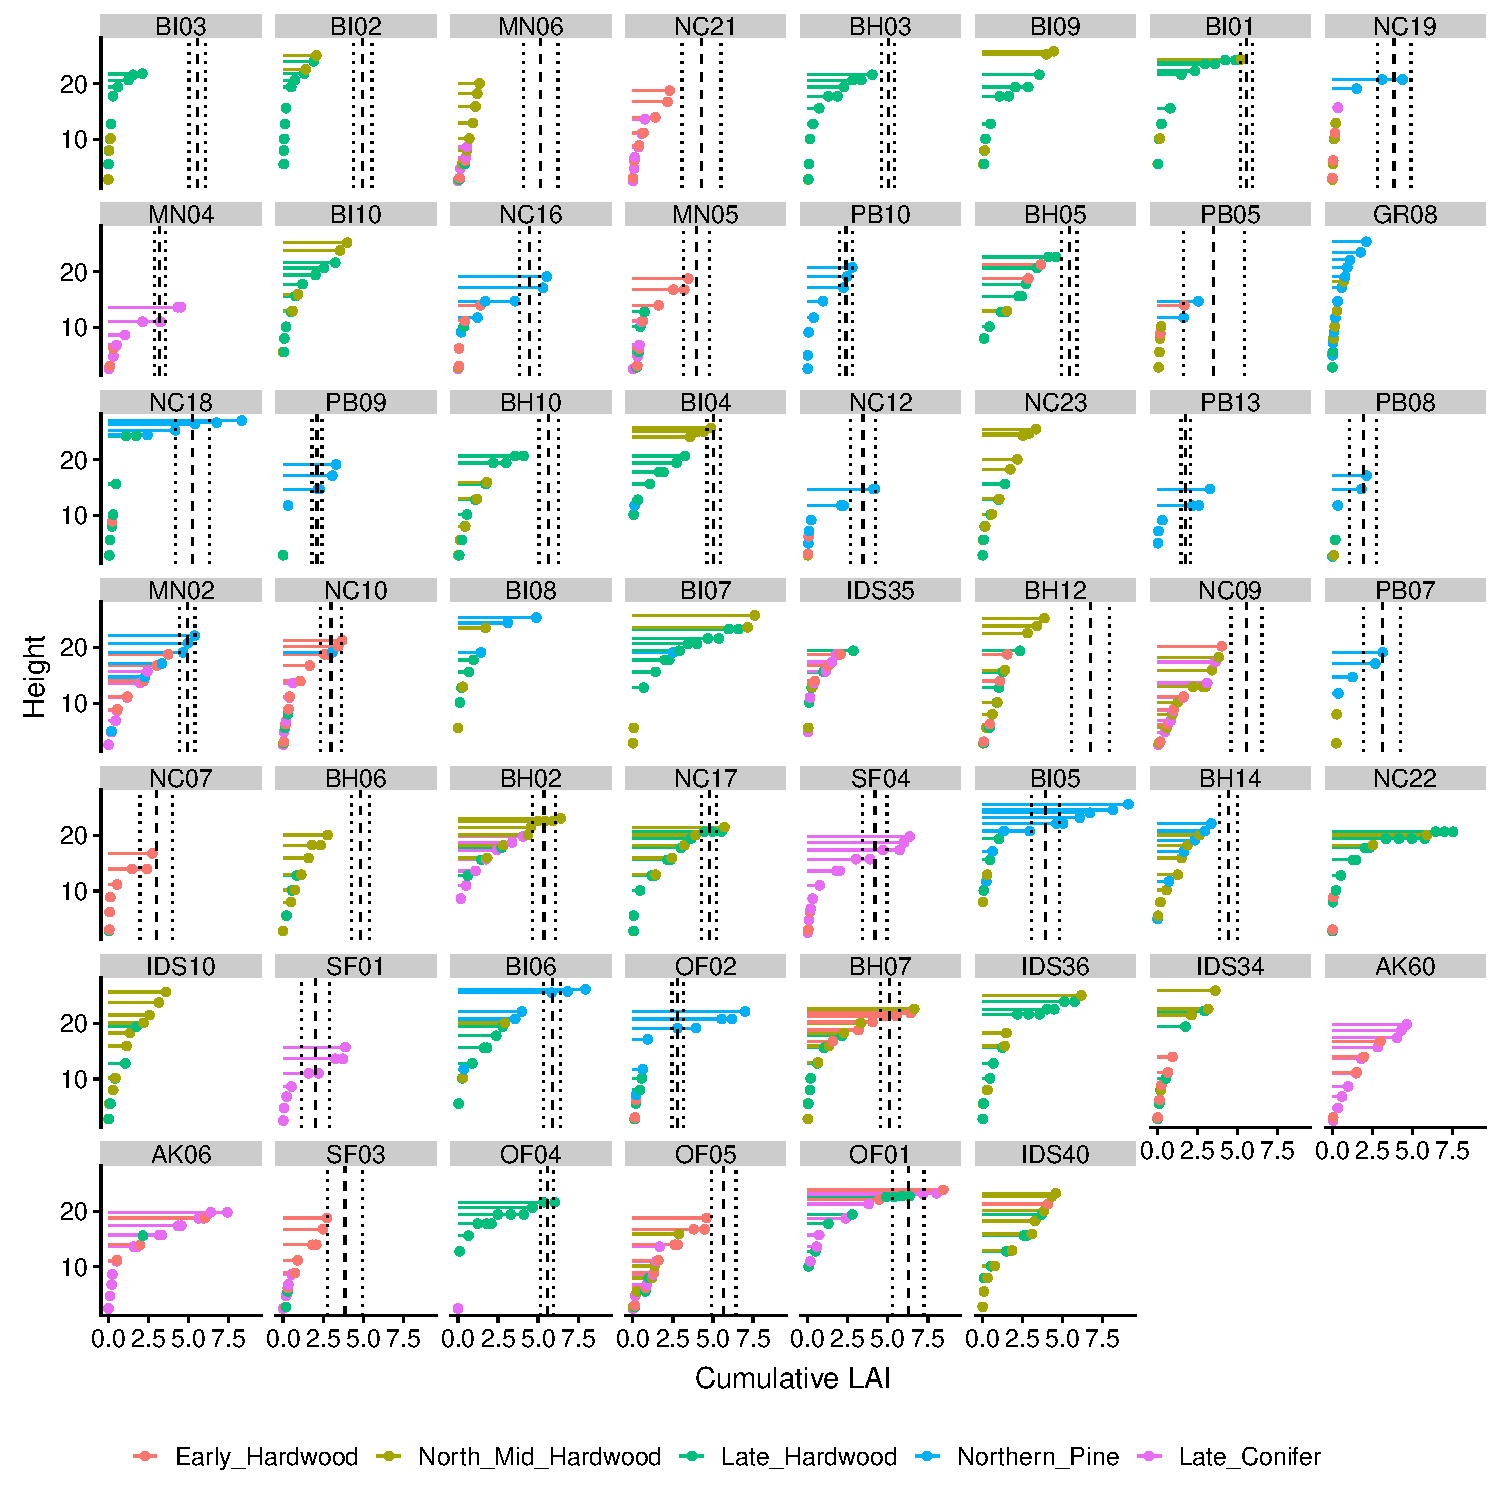
\includegraphics[width=\textwidth]{4_edr/figures/explore_spectra/ed_cumlai_plot.pdf}
  \caption{%
    Vertical profile of cumulative leaf area index and composition at each site in this analysis.
    Vertical black lines indicate the mean $\pm$ 1 standard deviation of the observed leaf area index.
    Sites are arranged in order of decreasing mean error in the visible range, as in Figures~\ref{fig:spec_error_all} and~\ref{fig:spec_error_vis}.
  }\label{fig:lai_profile}
\end{figure}

The ability of EDR to reproduce observed leaf area index was also strongly site-dependent, with some of the accuracy explained by the functional type of the tallest cohort (Figures~\ref{fig:lai_validation} and~\ref{fig:lai_profile}).
In general, EDR tended to over-predict leaf area index for conifer-dominated stands and under-predict for hardwood-dominated stands.
For mid- and late-hardwood-dominated stands in particular, EDR predicted substantial variability in leaf area index that was not present in the observations.

\subsection{Notes}

Positive bias in visible reflectance can largely be explained by wood reflectance.
Removing the wood reflectance eliminates most of the difference between SAIL and EDR.

Many of the sites where we get reflectance wrong are sites where late hardwood has a big presence.
In many other places, we get the LAI wrong.

Wood reflectance bias explains why we almost always miss the visible.

%\begin{figure}
  %\centering
  %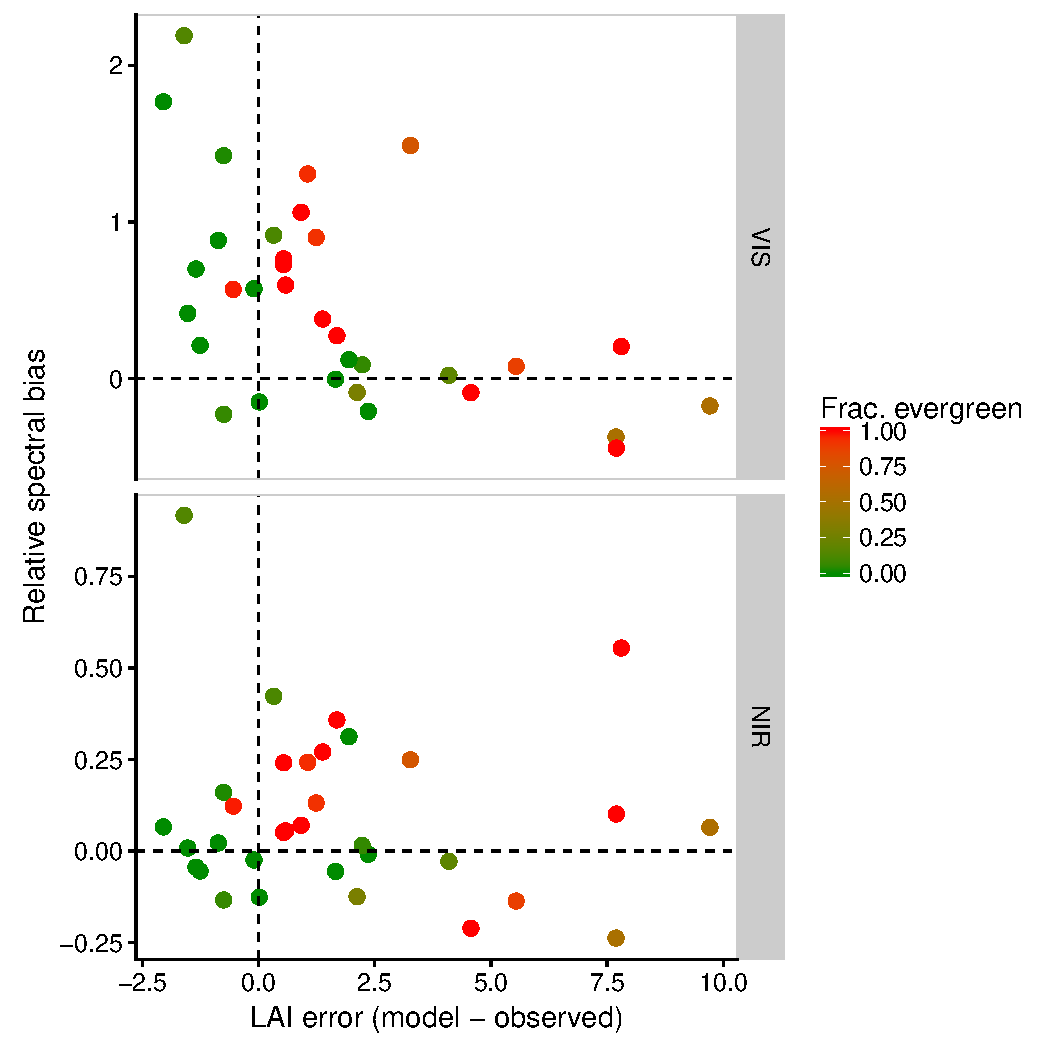
\includegraphics[width=\textwidth]{figures/spec_lai.pdf}
  %\caption{\
    %Relationship between errors in EDR predictions of leaf area index and spectra.
  %}\label{fig:spec_lai}
%\end{figure}

%There was a significant negative relationship between EDR LAI errors and spectral errors in the visible range;
%in other words, EDR tended to overestimate either LAI or canopy reflectance.

%\subsection{Forward simulation}
%\begin{figure}
  %\centering
  %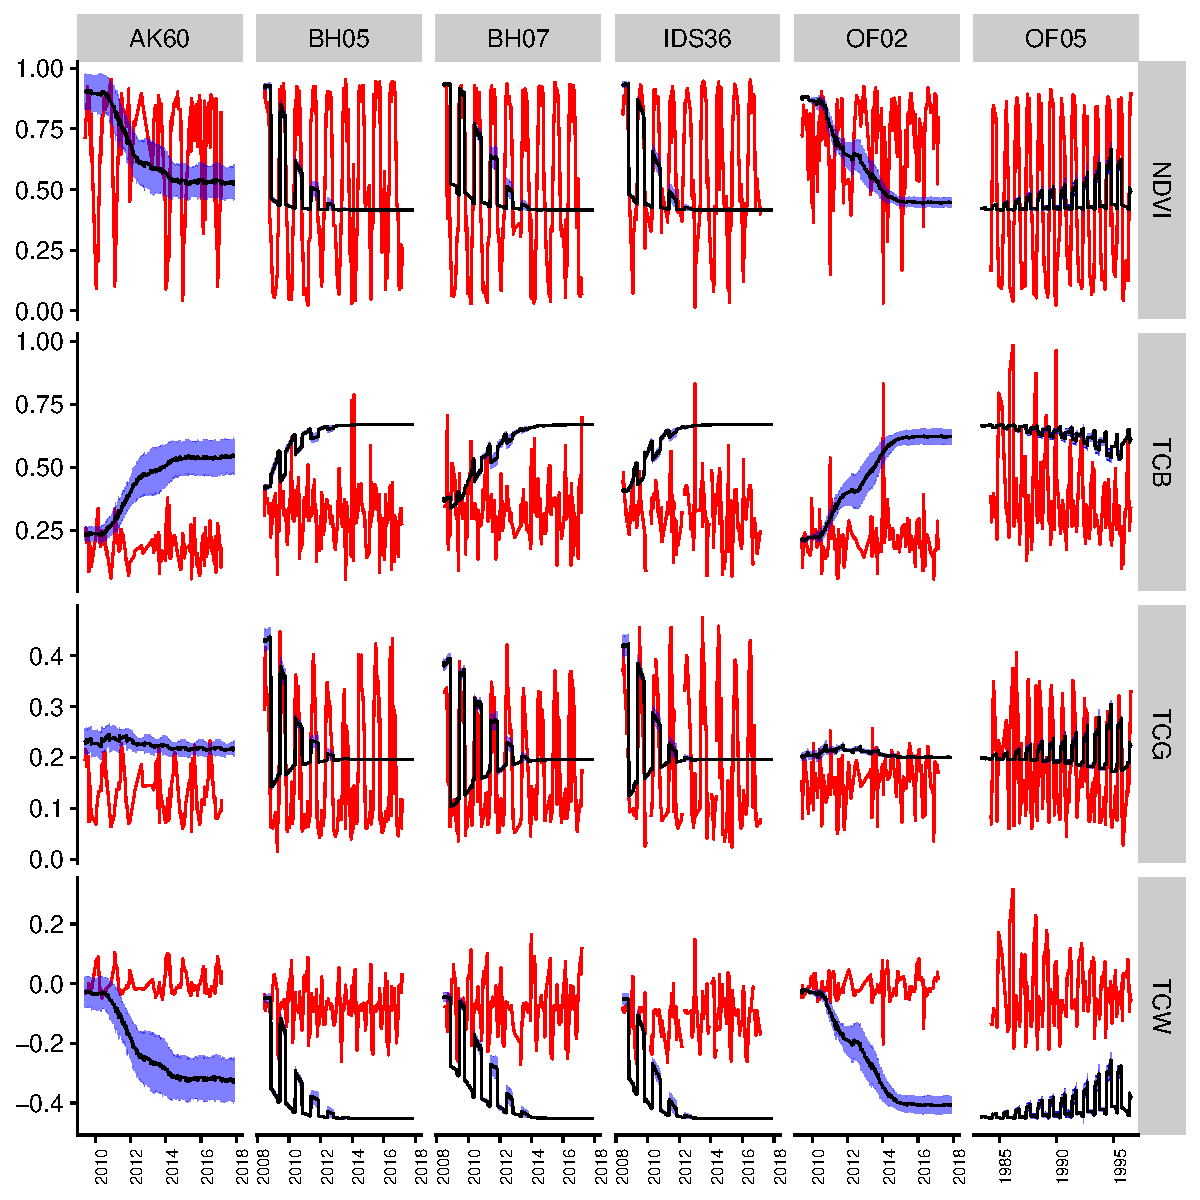
\includegraphics[width=\textwidth]{figures/landsat_ts.pdf}
  %\caption{\
    %Comparison of EDR-simulated (black, blue ribbon) and observed (red) time series of Landsat NDVI and tasseled cap brightness (TCB), greenness (TCG), and wetness (W) for each site.
  %}
%\end{figure}
%(Currently working on this text\ldots).
